\documentclass[aspectratio=169]{beamer}

\mode<presentation>
{
  \usetheme{default}
  \usecolortheme{default}
  \usefonttheme{default}
  \setbeamertemplate{navigation symbols}{}
  \setbeamertemplate{caption}[numbered]
  \setbeamertemplate{footline}[frame number]  % or "page number"
  \setbeamercolor{frametitle}{fg=white}
  \setbeamercolor{footline}{fg=black}
} 

\usepackage[english]{babel}
\usepackage[utf8x]{inputenc}
\usepackage{tikz}
\usepackage{courier}
\usepackage{array}
\usepackage{bold-extra}
\usepackage{minted}
\usepackage[thicklines]{cancel}

\xdefinecolor{dianablue}{rgb}{0.18,0.24,0.31}
\xdefinecolor{darkblue}{rgb}{0.1,0.1,0.7}
\xdefinecolor{darkgreen}{rgb}{0,0.5,0}
\xdefinecolor{darkgrey}{rgb}{0.35,0.35,0.35}
\xdefinecolor{darkorange}{rgb}{0.8,0.5,0}
\xdefinecolor{darkred}{rgb}{0.7,0,0}
\definecolor{darkgreen}{rgb}{0,0.6,0}
\definecolor{mauve}{rgb}{0.58,0,0.82}

\title[2018-02-28-iml-uproot]{\vspace{0.5 cm} \\ 
\includegraphics[width=0.25\linewidth]{uproot-logo.pdf} \\ Rapidly moving data from ROOT to Numpy and Pandas}
\author{Jim Pivarski}
\institute{Princeton University -- DIANA-HEP}
\date{February 28, 2018}

\begin{document}

\logo{\pgfputat{\pgfxy(0.11, 7.4)}{\pgfbox[right,base]{\tikz{\filldraw[fill=dianablue, draw=none] (0 cm, 0 cm) rectangle (50 cm, 1 cm);}\mbox{\hspace{-8 cm}
\includegraphics[height=1 cm]{princeton-logo-long.png}
\includegraphics[height=1 cm]{diana-hep-logo-long.png}}}}}

\begin{frame}
  \titlepage
\end{frame}

\logo{\pgfputat{\pgfxy(0.11, 7.4)}{\pgfbox[right,base]{\tikz{\filldraw[fill=dianablue, draw=none] (0 cm, 0 cm) rectangle (50 cm, 1 cm);}\mbox{\hspace{-8 cm}
\includegraphics[height=1 cm]{princeton-logo.png}
\includegraphics[height=1 cm]{diana-hep-logo.png}}}}}

% Uncomment these lines for an automatically generated outline.
%\begin{frame}{Outline}
%  \tableofcontents
%\end{frame}

% START START START START START START START START START START START START START

\begin{frame}{The what and why of uproot}
\vspace{0.5 cm}

\begin{block}{What is uproot?}
A pure Python $+$ Numpy implementation of ROOT I/O.
\end{block}

\vspace{0.5 cm}
\begin{block}{Why does it exist?}
\begin{enumerate}
\item To extract columnar data (branches) from a ROOT file without invoking the event-handling infrastructure of the ROOT framework.
\item As a faster and fewer-dependencies alternative to root\_numpy and root\_pandas.
\item To express the semantics and conventions of the ROOT file format independently of ROOT, in lieu of a formal specification.
\end{enumerate}
\end{block}
\end{frame}

\begin{frame}{Why reimplement ROOT I/O?}
\vspace{0.25 cm}
\begin{columns}
\column{0.73\linewidth}
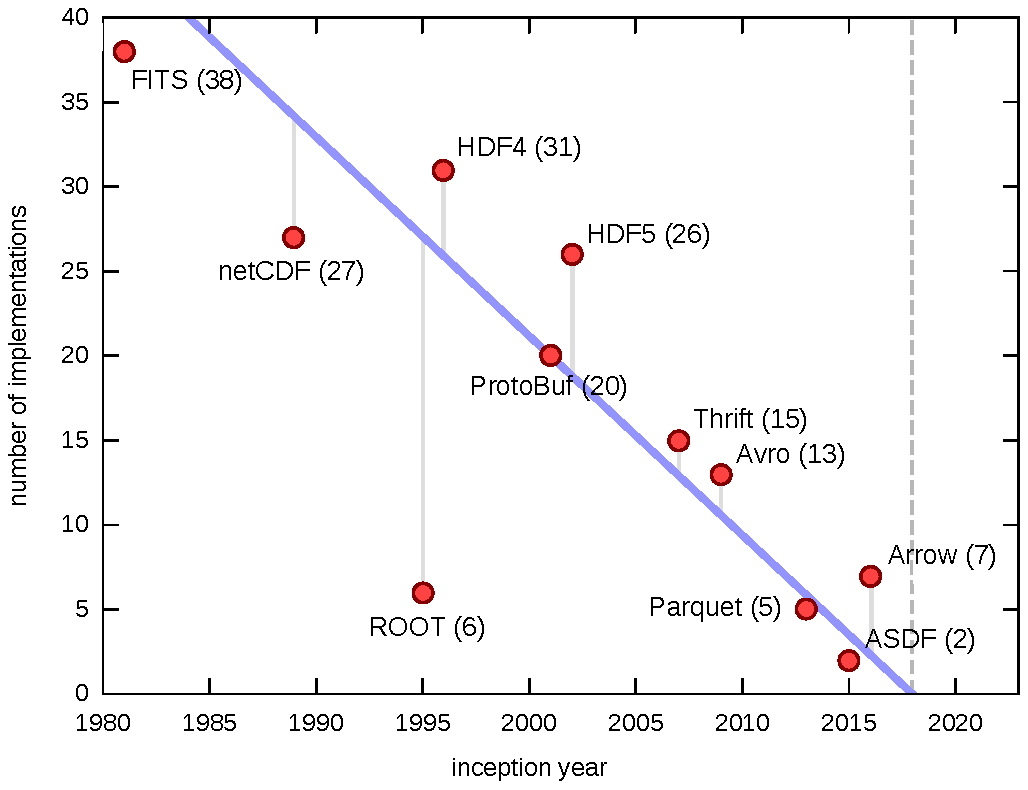
\includegraphics[width=\linewidth]{formats.pdf}
\column{0.25\linewidth}
It's more common to define a specification and implement many interpreters than not.

\vspace{0.25 cm}
Most connect the format to different contexts, such as different languages.

\vspace{0.25 cm}
\small\textcolor{gray}{(Take these numbers with a grain of salt: HDF5 is {\it criticized} because many of its bindings depend on only two C libraries!)}
\end{columns}
\end{frame}

\begin{frame}{ROOT I/O implementations}
\vspace{0.25 cm}
\begin{columns}
\column{1.2\linewidth}
\renewcommand{\arraystretch}{1.6}
\begin{tabular}{p{2.4 cm} c p{4.7 cm} p{5.25 cm}}
\centering ROOT & C++ & ROOT itself & The ROOT Team \\
\centering FreeHEP I/O $\to$ spark-root & Java/Scala & For Spark and other Big Data projects that run on Java & Started by Tony Johnson in 2001, updated by Viktor Khristenko \\
\centering RIO $\to$ inlib/exlib & C++ & Intended as an alternative, now embedded in GEANT-4 & Guy Barrand \\
\centering JsRoot & Javascript & For interacting with ROOT in web browsers or standalone & Bertrand Bellenot, Sergey Linev (in the ROOT Team) \\
\centering go-hep/rootio & Go & HEP analysis ecosystem in Go & Sebastien Binet \\
\centering \textcolor{blue}{uproot} & \textcolor{blue}{Python} & \textcolor{blue}{For quickly getting ROOT data into Numpy and Pandas for machine learning} & \textcolor{blue}{Jim Pivarski (me)} \\
alice-rs/root-io & Rust & ALICE ecosystem in Rust & Christian Bourjau \\
\end{tabular}
\end{columns}
\end{frame}

\begin{frame}{Why Python $+$ Numpy?}
\vspace{0.25 cm}
\begin{itemize}\setlength{\itemsep}{0.35 cm}
\item Physicists are already using Python for data analysis.

\begin{itemize}
\item \textcolor{gray}{PyROOT has excellent coverage of the ROOT ecosystem, but calling individually wrapped C++ methods from Python is slow and the two languages have different (often conflicting) memory management.}

\item \textcolor{gray}{Performance-oriented tools like root\_numpy and root\_pandas compile into a specific version of ROOT, which complicates upgrades. Also, asking for arrays through interfaces designed for event processing is a severe performance penalty.}
\end{itemize}

\item The scientific Python ecosystem, including much of machine learning, is designed around a fundamental abstraction called the Numpy array.

\item Working with computer scientists is easier when you can say, ``pip install uproot.''

\item Implemented correctly, Python $+$ Numpy doesn't have to be slow.

\begin{itemize}
\item \textcolor{gray}{Finding the columnar data in a ROOT file may be done in slow Python, as long as decompression and array manipulations are done by compiled code.}
\end{itemize}
\end{itemize}
\end{frame}

\begin{frame}{More context: BulkIO}
\vspace{0.75 cm}
\begin{center}
\begin{minipage}{0.8\linewidth}
Last summer, Brian Bockelman started a project called ``BulkIO'' to bypass the event processing framework in ROOT itself, providing direct access to branches as columns.

\vspace{0.75 cm}
I added a BulkIO-to-Numpy interface in PyROOT in the same pull request [\textcolor{blue}{\href{https://github.com/root-project/root/pull/943}{\#943}}] and intend to maintain it, when it's approved.

\vspace{0.75 cm}
I wrote uproot while the pull request is in progress, based on the same BulkIO technique.
\end{minipage}
\end{center}
\end{frame}

\begin{frame}{}
\begin{center}
\Huge \textcolor{darkblue}{A tour of uproot}
\end{center}
\end{frame}

\begin{frame}[fragile]{A tour of uproot}
\vspace{0.35 cm}
\small

{\normalsize Install uproot and download a sample file.}

\begin{minted}{bash}
$ pip install uproot --user
$ wget http://scikit-hep.org/uproot/examples/Zmumu.root
\end{minted}

\vspace{0.2 cm}
{\normalsize Start using it in Python.}

\begin{minted}{python3}
>>> import uproot
>>> file = uproot.open("Zmumu.root")  # or root:// or http://
\end{minted}

\vspace{0.2 cm}
{\normalsize ROOT files, directories, and trees are like Python dicts with {\tt\small keys()} and {\tt\small values()}.}

\begin{minted}{python3}
>>> file.keys()
['events;1']
>>> tree = file["events"]
>>> tree.keys()
['Type', 'Run', 'Event', 'E1', 'px1', 'py1', 'pz1', 'pt1', 'eta1',
 'phi1', 'Q1', 'E2', 'px2', 'py2', 'pz2', 'pt2', 'eta2', 'phi2',
 'Q2', 'M']
\end{minted}
\end{frame}

\begin{frame}[fragile]{A tour of uproot}
\vspace{0.5 cm}
\small

{\normalsize uproot's main purpose is to read branches from ROOT files as Numpy arrays.}

\begin{minted}{python3}
>>> tree["px1"].array()
array([-41.195287,  35.118049,  35.118049, ...,  32.377491,
        32.377491,  32.485393])

>>> tree.arrays(["px1", "py1", "pz1"])
{'px1': array([-41.195287,  35.118049,  35.118049, ...,  32.377491,
                32.377491,  32.485393]),
 'py1': array([ 17.43324 , -16.570362, -16.570362, ...,   1.199405,
                 1.199405,   1.20135 ]),
 'pz1': array([-68.964961, -48.775246, -48.775246, ..., -74.532430,
               -74.532430, -74.808372])}
\end{minted}
\end{frame}

\begin{frame}[fragile]{A tour of uproot}
\vspace{0.5 cm}
\small

{\normalsize Iteration lets us fetch data in batches--- large enough to be efficient in Python but small enough to fit in memory.}

\begin{minted}{python3}
>>> for arrays in tree.iterate(entrysteps=10000):
...     do_something(arrays)   # all arrays in chunks of 10k events

>>> for arrays in uproot.iterate("/path/to/files*.root", "Events"):
...     do_something(arrays)   # this is like a TChain
\end{minted}

\vspace{0.2 cm}
{\normalsize The array-fetching methods share most parameters: you can specify a subset of branches in {\tt\small iterate} just as you would in {\tt\small arrays}.}

\vspace{0.2 cm}
{\normalsize If unspecified, {\tt\small entrysteps} defaults to the ROOT file's cluster size, reading whole baskets at a time.}
\end{frame}

\begin{frame}[fragile]{A tour of uproot}
\vspace{0.5 cm}
\small

{\normalsize One of these array-fetching methods fills a Pandas DataFrame.}

\begin{minted}{python3}
>>> tree.pandas.df(["pt*", "eta*", "phi*"])
          eta1      eta2      phi1      phi2      pt1      pt2
0    -1.217690 -1.051390  2.741260 -0.440873  44.7322  38.8311
1    -1.051390 -1.217690 -0.440873  2.741260  38.8311  44.7322
2    -1.051390 -1.217690 -0.440873  2.741260  38.8311  44.7322
3    -1.051390 -1.217690 -0.440873  2.741260  38.8311  44.7322
...        ...       ...       ...       ...      ...      ...
2300 -1.482700 -1.570440 -2.775240  0.037027  72.8781  32.3997
2301 -1.570440 -1.482700  0.037027 -2.775240  32.3997  72.8781
2302 -1.570440 -1.482700  0.037027 -2.775240  32.3997  72.8781
2303 -1.570440 -1.482700  0.037027 -2.775240  32.3997  72.8781

[2304 rows x 6 columns]
\end{minted}

\vspace{0.2 cm}
{\normalsize Features like this are easy now that the core ROOT-reading functionality is in place.}
\end{frame}

\begin{frame}[fragile]{A tour of uproot}
\vspace{0.5 cm}
\small

{\normalsize uproot follows Pythonic customs: high-level yet explicit. For example, asking for the same array twice reads it from the file twice.}

\begin{minted}{python3}
>>> arrays = tree.arrays()               # reads all data
>>> arrays = tree.arrays()               # reads all data again
\end{minted}

\vspace{0.2 cm}
{\normalsize That is, unless you give it a cache (anything that acts like a dict).}

\begin{minted}{python3}
>>> cache = {}
>>> arrays = tree.arrays(cache=cache)    # reads all data
>>> arrays = tree.arrays(cache=cache)    # gets it from the cache
>>> len(cache)
20

>>> limitedcache = uproot.cache.MemoryCache(5*1024)   # limit to 5 kB
>>> arrays = tree.arrays(cache=limitedcache)
>>> len(limitedcache)
18
\end{minted}
\end{frame}

\begin{frame}[fragile]{A tour of uproot}
\label{page:executor}\vspace{0.5 cm}
\small

{\normalsize Same for concurrency: it's single-threaded unless you give it an executor (anything with a {\tt\small map} method returning a non-blocking generator of results).}

\begin{minted}{python3}
>>> from concurrent.futures import ThreadPoolExecutor

>>> executor = ThreadPoolExecutor(8)           # 8 threads
>>> arrays = tree.arrays(executor=executor)    # read, decompress all
                                               # baskets in parallel
\end{minted}

\vspace{0.2 cm}
{\normalsize There's also a non-blocking form that returns a function. Processing happens in the background until you call this function, which waits for and returns the array data.}

\begin{minted}{python3}
>>> wait = tree.arrays(executor=executor, blocking=False)
>>> wait
<function wait at 0x7a1d744515f0>
>>> wait()                                     # now get the arrays
...
\end{minted}
\end{frame}

\begin{frame}[fragile]{A tour of uproot}
\vspace{0.4 cm}
\small

{\normalsize A lot of ROOT trees are not flat tables, but contain arbitrary-length lists of particle attributes. Numpy only deals with n-dimensional arrays, so we need a new container.}

\begin{minted}{python3}
>>> tree = uproot.open("http://scikit-hep.org/uproot/"
...                           "examples/HZZ.root")["events"]
>>> ja = tree.array("Jet_E")
>>> ja
jaggedarray([[],
             [44.137363],
             [],
             ...,
             [55.95058],
             [229.57799  33.92035],
             []])
>>> ja[0]
array([], dtype=float32)
>>> ja[1]
array([44.137363], dtype=float32)
\end{minted}
\end{frame}

\begin{frame}[fragile]{A tour of uproot}
\vspace{0.4 cm}
\small

{\normalsize This is much faster than root\_numpy's behavior (arrays as objects in an object array) because uproot only loads the information needed to identify subarrays (contiguous in memory) without constructing them all (randomly in memory).}

\begin{minted}{python3}
>>> ja.content
array([44.13, 230.34, 101.35 ... 55.95, 229.57, 33.92], dtype=float32)
>>> ja.offsets
array([0, 0, 1 ... 2771, 2773, 2773])
\end{minted}

\vspace{0.2 cm}
{\normalsize There are also string types, vector of strings, vector of vector of numbers, etc. Eventually, uproot will be able to interpret any data type. To see if your branch's type is currently supported, call {\tt\small tree.show()} and check the third column for {\tt\small None}.}

\begin{minted}{python3}
>>> tree.show()
NJet                (no streamer)       asdtype('>i4')
Jet_E               (no streamer)       asjagged(asdtype('>f4'))
Jet_ID              (no streamer)       asjagged(asdtype('>bool'))
...
\end{minted}
\end{frame}

\begin{frame}[fragile]{A tour of uproot}
\vspace{0.35 cm}
\scriptsize

\begin{columns}
\column{1.1\linewidth}
{\normalsize uproot uses a ROOT file's streamer info to know how to deserialize classes, staying abreast of changes. Thus, any type of object may be extracted from a ROOT file.}

\begin{minted}{bash}
$ wget "https://github.com/HEPData/hepdata-submission/blob/master/examples/submission/"\
"TestHEPSubmission/root_file.root?raw=true" -O hepdata.root
\end{minted}

\begin{minted}{python3}
>>> file = uproot.open("hepdata.root")
>>> dict(file.classes())
{'hpx;1': <class uproot.rootio.TH1F>, 'hpxpy;1': <class uproot.rootio.TH2F>,
 'hprof;1': <class uproot.rootio.TProfile>, 'ntuple;1': <class uproot.rootio.TNtuple>}
>>> histogram = file["hpx"]
>>> histogram.fTitle
'This is the px distribution'
>>> histogram.fFunctions[0]
<TPaveStats 'stats' at 0x71cb4586df90>
\end{minted}
\begin{minted}{python3}
>>> histogram.fXaxis.__dict__           # all the fields are there, without interpretation
{'fTitleFont': 42, 'fLabelColor': 1, 'fNdivisions': 510, 'fXmin': -4.0,
 'fTimeDisplay': False, 'classversion': 1, 'fLabelFont': 42, 'fNbins': 100,
 'fLabels': None, 'fXbins': [], 'fTitleColor': 1, 'fLabelOffset': 0.004999999888241291,
 'fName': 'xaxis', 'fLast': 0, 'fAxisColor': 1, 'fLabelSize': 0.03500000014901161,
 'fTitleOffset': 1.0, 'fTitle': '', 'fFirst': 0, 'fXmax': 4.0,
 'fTickLength': 0.029999999329447746, 'fTimeFormat': '', 'fBits2': 0,
 'fTitleSize': 0.03500000014901161}
\end{minted}
\end{columns}
\end{frame}

\begin{frame}[fragile]{A tour of uproot}
\vspace{0.4 cm}
\scriptsize

{\normalsize All that remains is to give these objects Pythonic interpretations.}

\begin{minted}{python3}
>>> histogram.bokeh.plot()            # basic implementation, somewhat clunky
>>> histogram.holoviews.plot()        # only works in a Jupyter notebook

>>> histogram.fit(lambda x, a, b, c: a*exp(-(x - b)**2 / c))    # dreaming...

>>> histogram.show()                  # surprisingly useful
                  0                                                       2410.8
                  +------------------------------------------------------------+
[-inf, -3)   0    |                                                            |
[-3, -2.4)   68   |**                                                          |
[-2.4, -1.8) 285  |*******                                                     |
[-1.8, -1.2) 755  |*******************                                         |
[-1.2, -0.6) 1580 |***************************************                     |
[-0.6, 0)    2296 |*********************************************************   |
[0, 0.6)     2286 |*********************************************************   |
[0.6, 1.2)   1570 |***************************************                     |
[1.2, 1.8)   795  |********************                                        |
[1.8, 2.4)   289  |*******                                                     |
[2.4, 3)     76   |**                                                          |
[3, inf]     0    |                                                            |
                  +------------------------------------------------------------+
\end{minted}
\end{frame}

\begin{frame}{}
\begin{center}
\Huge \textcolor{darkblue}{Performance}
\end{center}
\end{frame}

\begin{frame}{Performance: comparison to root\_numpy (uncompressed)}
\vspace{0.4 cm}

In terms of functionality, uproot is most similar to root\_numpy. Depending on basket size and whether the array is flat (fixed width per event) or jagged (variable width), uproot can be as much as 40 times faster.

\begin{columns}
\column{1.15\linewidth}
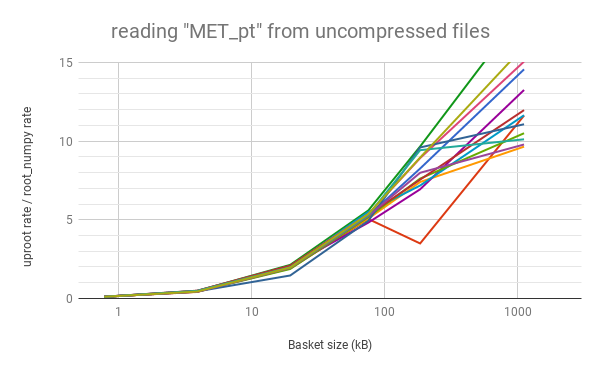
\includegraphics[width=0.5\linewidth]{rootnumpy-none-met.png}
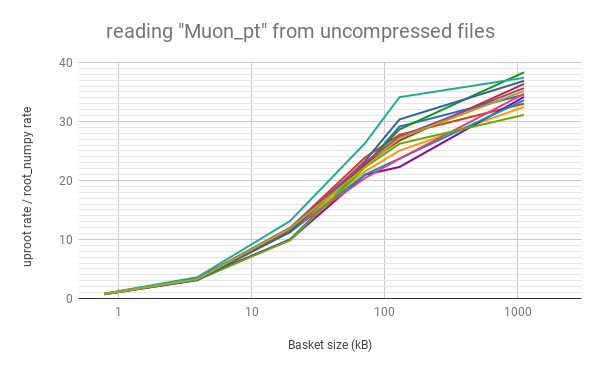
\includegraphics[width=0.5\linewidth]{rootnumpy-none-muon.png}
\end{columns}

The 13 lines are different physics distributions from CMS NanoAOD (mileage varies). Speedup increases with basket size because more work is done in Numpy, not Python.
\end{frame}

\begin{frame}{Performance: comparison to root\_numpy (gzip-compressed)}
\vspace{0.5 cm}

The distinction drops to a factor of 3 when flat data are compressed, but still there's a factor of 10 for jagged data because of the way root\_numpy handles this type.

\vspace{0.5 cm}
\begin{columns}
\column{1.15\linewidth}
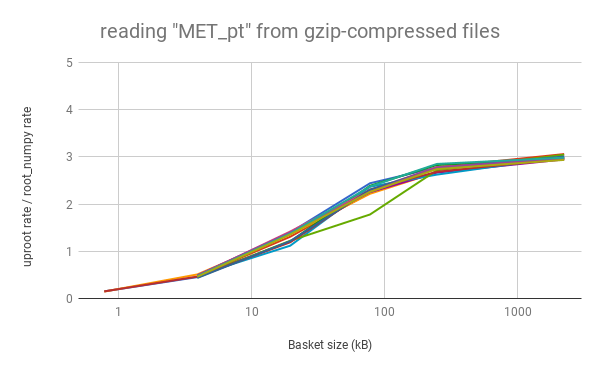
\includegraphics[width=0.5\linewidth]{rootnumpy-gzip-met.png}
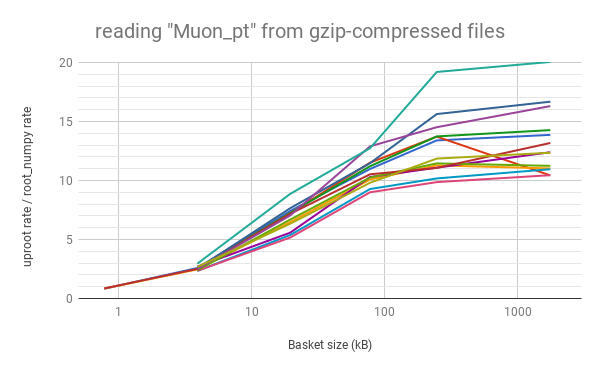
\includegraphics[width=0.5\linewidth]{rootnumpy-gzip-muon.png}
\end{columns}
\end{frame}

\begin{frame}{Performance: comparison to ROOT (uncompressed)}
\vspace{0.5 cm}

For sufficiently large baskets, uproot even compares favorably to ROOT because uproot bypasses the event processing framework.

\vspace{0.25 cm}
\begin{columns}
\column{1.15\linewidth}
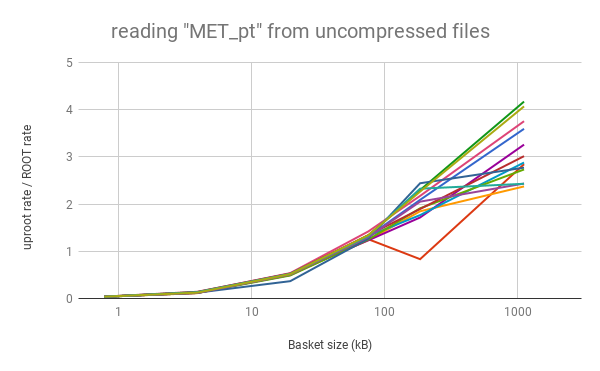
\includegraphics[width=0.5\linewidth]{root-none-met.png}
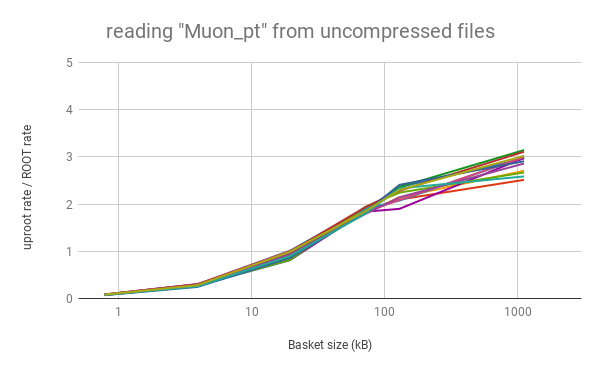
\includegraphics[width=0.5\linewidth]{root-none-muon.png}
\end{columns}

\vspace{0.25 cm}
When the BulkIO feature is added to ROOT, it will be about 30 times faster than this baseline, so ROOT {\tt\small TBranch::GetEntry} $\ll$ uproot $\ll$ ROOT BulkIO.
\end{frame}

\begin{frame}{Performance: comparison to ROOT (gzip-compressed)}
\vspace{0.5 cm}
As you add compression, the distinction washes out because both processes spend more of their time in the same decompression algorithm.

\vspace{0.25 cm}
\begin{columns}
\column{1.15\linewidth}
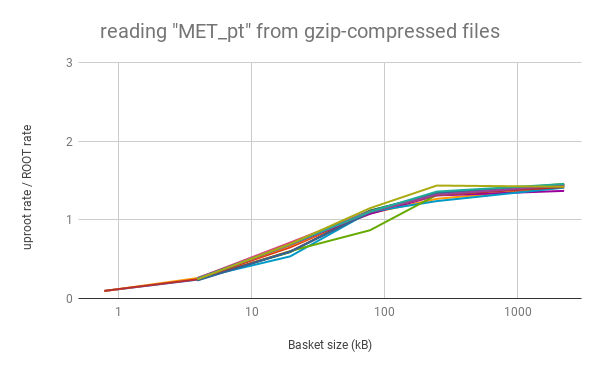
\includegraphics[width=0.5\linewidth]{root-gzip-met.png}
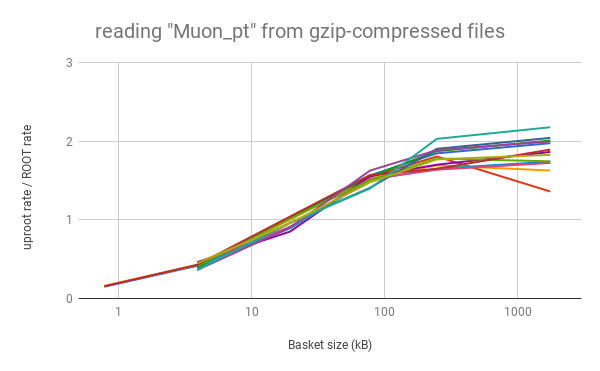
\includegraphics[width=0.5\linewidth]{root-gzip-muon.png}
\end{columns}

\vspace{0.25 cm}
For read performance, no compression $\sim$ lz4 $\ll$ gzip $\ll$ lzma.
\end{frame}

\begin{frame}[fragile]{If you are preparing data for uproot}
\vspace{0.5 cm}
\small

{\normalsize \ldots make large baskets:}

\begin{minted}{c++}
// 100 kB to 1 MB baskets
tree->Branch("branch", &data, "branch/F", 1024*1024);

// negative flush size is size of all branches in a cluster
tree->SetAutoFlush(-1024*1024 * numbranches);
\end{minted}

\vspace{0.75 cm}
{\normalsize \ldots and use LZ4 compression:}

\begin{minted}{c++}
file->SetCompressionAlgorithm(ROOT::kLZ4);    // ROOT::kLZ4 is 4
file->SetCompressionLevel(3);
\end{minted}
\end{frame}

\begin{frame}{Last performance plot: multithreaded scaling}
\vspace{0.5 cm}
Although Python locks all threads at each step in its interpreter (the ``GIL''), compiled code escapes this limitation and can scale on multicore machines.

\begin{center}
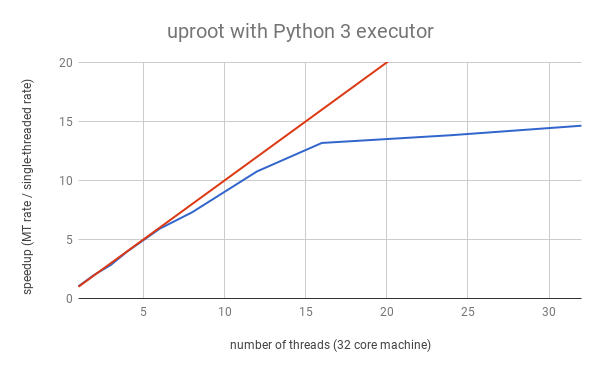
\includegraphics[width=0.65\linewidth]{scaling.png}
\end{center}

In the above, we iterated through a thousand lzma-compressed branches (lzma requires the most CPU time to decompress), distributed as described on page~\pageref{page:executor}.
\end{frame}

\begin{frame}{}
\begin{center}
\Huge \textcolor{darkblue}{Activity, status, and future}
\end{center}
\end{frame}

\begin{frame}{Download statistics (via ``pip install'')}
\vspace{0.25 cm}

\begin{columns}
\column{1.06\linewidth}
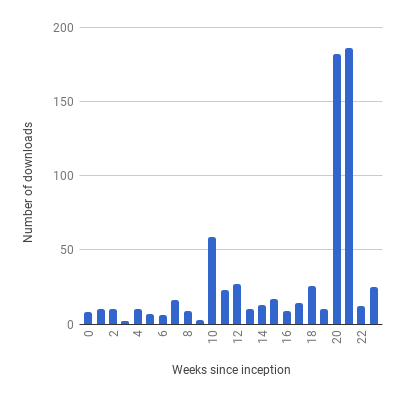
\includegraphics[width=0.34\linewidth]{downloads-vs-week.png}
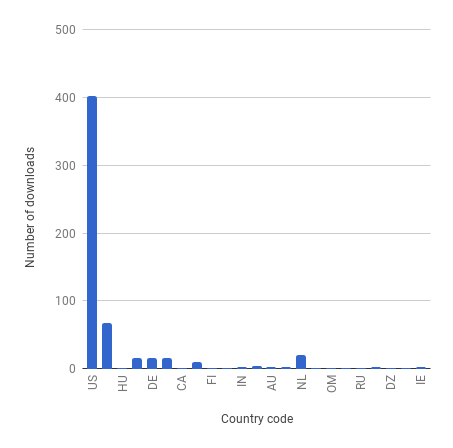
\includegraphics[width=0.34\linewidth]{downloads-vs-country.png}
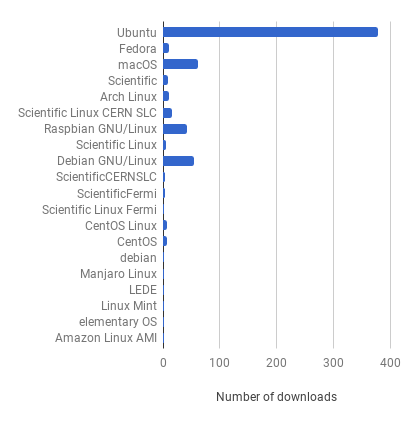
\includegraphics[width=0.33\linewidth]{downloads-vs-os.png}
\end{columns}

\vspace{0.25 cm}
Number of unique country code/OS distribution/version combinations (``users''): 127.

\vspace{0.1 cm}
Client in NL requests every version; others request only the latest.

\vspace{0.1 cm}
Popular with Linux laptops (Ubuntu); I want to know who's using it on a Raspberry Pi!

\vspace{0.1 cm}
GitHub issues not posted by me: 33; \ stars: 72; \ watchers: 10.
\end{frame}

\begin{frame}{Status and future}
\vspace{0.5 cm}
\begin{center}
\begin{minipage}{0.95\linewidth}
\large
\begin{itemize}\setlength{\itemsep}{0.5 cm}
\item uproot has reached a stable plateau, I'm mostly responding to bugs and feature requests now--- no deep overhauls.
\item This summer, Pratyush Das (an undergrad) will be adding write support for file output.
\item uproot will always be an I/O-only library. However, it may accrue features that {\it connect} it to other packages, such as

\vspace{0.2 cm}
{\tt\small \hspace{1 cm}tree.pandas.df()}

\vspace{0.2 cm}
and

\vspace{0.2 cm}
{\tt\small \hspace{1 cm}histogram.bokeh.plot()}

\vspace{0.2 cm}
which can eventually make it part of a Pythonic analysis environment.
\end{itemize}
\end{minipage}
\end{center}
\end{frame}

\begin{frame}{Status and future}
\vspace{0.5 cm}
\begin{center}
\begin{minipage}{0.8\linewidth}
Yesterday, Chris Burr implemented a pyparsing-based translator from ROOT's TFormula language to numexpr. This would make it possible for uproot to reproduce all functionality currently found in root\_numpy.

\vspace{0.5 cm}
Is there interest in
\begin{center}
\tt import uproot.root\_numpy as root\_numpy
\end{center}
as a drop-in replacement?
\end{minipage}
\end{center}
\end{frame}

\begin{frame}[fragile]{Last slide: thanks for listening!}
\vspace{0.5 cm}
\huge
\begin{center}
\begin{minipage}{0.8\linewidth}
\begin{verbatim}
pip install uproot --user
\end{verbatim}
\end{minipage}

\Large
\vspace{1 cm}
\href{https://github.com/scikit-hep/uproot}{\textcolor{blue}{https://github.com/scikit-hep/uproot}}

\vspace{0.5 cm}
\href{http://uproot.readthedocs.io}{\textcolor{blue}{http://uproot.readthedocs.io}}

\vspace{0.5 cm}
\href{https://groups.google.com/forum/#!forum/uproot-users/join}{\textcolor{blue}{https://groups.google.com/forum/\#!forum/uproot-users/join}}
\end{center}
\end{frame}

\begin{frame}{}
\begin{center}
\Huge \textcolor{darkblue}{BACKUP}
\end{center}
\end{frame}

\begin{frame}[fragile]{Code used for performance studies}
\vspace{0.5 cm}
\scriptsize

{\normalsize For all (prewarmed cache eliminates dependence on disk, which was SSD anyway):}

\begin{minted}{bash}
$ vmtouch -t filename
\end{minted}

\vspace{0.5 cm}
\mbox{ } \hfill \begin{minipage}{0.5\linewidth}
{\normalsize For uproot:}

\begin{minted}{python3}
import uproot
tree = uproot.open(filename)[treename]

startTime = time.time()
tree.array(branchname)
return time.time() - startTime
\end{minted}
\end{minipage} \hfill \mbox{ }

\vspace{0.5 cm}
\hfill \begin{minipage}{0.5\linewidth}
{\normalsize For root\_numpy:}

\begin{minted}{python3}
import root_numpy
file = ROOT.TFile(filename)
tree = file.Get(treename)

startTime = time.time()
root_numpy.tree2array(tree, [branchname])
return time.time() - startTime
\end{minted}
\end{minipage}
\end{frame}

\begin{frame}[fragile]{Code used for performance studies}
\vspace{0.25 cm}
\scriptsize

\begin{columns}[b]
\column{0.5\linewidth}
{\normalsize For C++ ROOT:}

\begin{minted}{c++}
TFile *file = new TFile(filename);
TTree *tree;
file->GetObject(treename, tree);

float MET_pt;
float Muon_pt[8];

TBranch *branch;
if (branchname == "Muon_pt") {
  branch = treein->GetBranch("Muon_pt");
}
else if (branchname == "MET_pt") {
  branch = treein->GetBranch("MET_pt");
}

branch->SetAddress(&MET_pt);
branch->SetAddress(&Muon_pt);
\end{minted}

\column{0.55\linewidth}
\begin{minted}{c++}
struct timeval startTime, endTime;

Long64_t nEvents = tree->GetEntries();
Long64_t iEvent;
gettimeofday(&startTime, 0);
for (iEvent = 0; iEvent < nEvents; ++iEvent) {
    // not tree->GetEntry(iEvent) because
    // that would touch all branches!
    branch->GetEntry(iEvent);
}
gettimeofday(&endTime, 0);

double microsecs =
   1000000*(endTime.tv_sec - startTime.tv_sec)
         + (endTime.tv_usec - startTime.tv_usec);

return microsecs / 1000000.0;
\end{minted}
\end{columns}
\end{frame}

\end{document}
